\chapter{Implémentation de l'algorithme BSO pour le problème SAT}
	\section{Structures de données:}
	\paragraph{}
	Comme vu dans l’approche par espace des états la représentation du problème et les structures de données ont un impact considérable sur les performances de l’implémentation d’un algorithme.\\
	Dans cette partie nous allons voir les structures de données adéquates à notre implémentation de BSO.
	\subsection{Représentation d’instance et de solutions SAT:}
	\paragraph{}
	Nous allons utilisé la représentation par Bitset vu précédemment dans laquelle on représente une instance SAT en gardant pour chaque littéral les clauses qu’il satisfait dans un Bitset, et une solution SAT par un Bitset de taille égale au nombre de variables de l’instance SAT et pour chaque variable on lui associe un bit qui est met à 1 si la variable est vrai, à 0 sinon.
	Pour résumé tout cela, soit l’instance SAT suivante:
	\begin{flalign*}
	x_{1} \lor \neg x_{2} \lor x_{4} \\
	\neg x_{2} \lor x_{3} \lor x_{4} \\
	\neg x_{1} \lor x_{2} \lor \neg x_{3}
	\end{flalign*}
	Et la solution suivante:\\
	\begin{center}
		$x_{1} \leftarrow true$, $x_{2} \leftarrow false$, $x_{3} \leftarrow true$, $x_{4} \leftarrow false $
	\end{center}
	
	La représentation:\\
	
	\definecolor{green}{rgb}{0.5,1,0.5}
	\begin{center}
		\begin{tabular}{|c | c| c| c| c|}
			\hline
			$x_{1}$& $x_{2}$ &$x_{3}$ &$x_{4}$ \\\hline
			1 & 0 & 1 & 0 \\\hline
		\end{tabular}\\
		Solution
	\end{center}
	\begin{minipage}{0.5\textwidth}
		\centering
		\begin{tabular}{|c | c| c| c|}
			\hline
			\rowcolor{green}
			$x_{1}$& 1 & 0 & 0 \\\hline
			$x_{2}$& 0 & 0 & 1 \\\hline
			\rowcolor{green}
			$x_{3}$& 0 & 1 & 0 \\\hline
			$x_{4}$& 1 & 1 & 0 \\\hline
		\end{tabular}
	\end{minipage}
	\hfillx
	\begin{minipage}{0.5\textwidth}
		\centering
		\begin{tabular}{|c | c| c| c|}
			\hline
			$\neg x_{1}$& 0 & 0 & 1 \\\hline
			\rowcolor{green}
			$\neg x_{2}$& 1 & 1 & 0 \\\hline
			$\neg x_{3}$& 0 & 0 & 1 \\\hline
			\rowcolor{green}
			$\neg x_{4}$& 0 & 0 & 0 \\\hline
		\end{tabular}
	\end{minipage}\\
	\begin{center}
		Instance
	\end{center}
	On peut calculer les clauses satisfaites par la solution en utilisant le or logique entre les Bitset de ses littéraux:
	\begin{center}
		\begin{minipage}{0.5\textwidth}
			\centering
			\begin{tabular}{| c| c| c|c|}
				\hline
				$x_{1}$& 1 & 0 & 0 \\\hline
			\end{tabular}
		\end{minipage}
		\\~\\
		OR
		\\~\\
		\begin{minipage}{0.5\textwidth}
			\centering
			\begin{tabular}{|c | c| c| c|}
				\hline
				$x_{3}$& 0 & 1 & 0 \\\hline
			\end{tabular}
		\end{minipage}
		\\~\\
		OR
		\\~\\
		\begin{minipage}{0.5\textwidth}
			\centering
			\begin{tabular}{| c| c| c|c|}
				\hline
				$\neg x_{2}$& 1 & 1 & 0 \\\hline
			\end{tabular}
		\end{minipage}
		\\~\\
		OR
		\\~\\
		\begin{minipage}{0.5\textwidth}
			\centering
			\begin{tabular}{|c | c| c| c|}
				\hline
				$\neg x_{4}$& 0 & 0 & 0 \\\hline
			\end{tabular}
		\end{minipage}
		\begin{center}
			
			$\downarrow$
			\\~\\
			\begin{tabular}{|c | c| c| c|}
				\hline
				$Bitset$ résultat& 1 & 1 & 0 \\\hline
			\end{tabular}
		\end{center}
	\end{center}
	
	
	\subsection{La table Dance:}
	\paragraph{}
	Comme la plupart des méta-heuristique, BSO travaille sur une solution qu’il essaye d’améliorer à chaque itération. Une table contenant les meilleures solutions, appelée Dance, est utilisée. Nous avons opté à organiser cette table sous forme de tas, ainsi à chaque itération la racine du tas est choisie pour le traitement, suite à cela, les meilleures solutions trouvées par les abeilles à la fin de l’itération sont insérées dans la table.
	\section{Conception et pseudo-code:}
	\paragraph{}
	Nous présentons dans la suite les parties essentielles constituant la méthode BSO.
	\subsection{Algorithme de recherche:}
	Comme expliqué précédemment, à chaque itération on essaye d’améliorer une solution initiale. L’itération commence par générer des solution équidistante de la solution initial, et pour chaque solution générée on fait une recherche locale. Ensuite, chacune des solutions trouvées localement est insérées dans la table Dance cité précédemment. L’itération suivante fera le même traitement en commençant par la meilleure solution de Dance. Cela est répété jusqu’à ce qu'on arrive à la solution optimale ou à une condition d’arrêt, nombre maximum d’itération atteint par exemple.
	\begin{algorithm}
		\SetAlgoLined
		\KwResult{retourne la meilleure solution trouvée}
		$sRef \gets $\textbf{solution aléatoire}\;
		$meilleureSolution \gets sRef$\;
		\While{$\neg$\textbf{fin()}}{
			\textbf{ajouter($listeTabou$,$sRef$)}\;
			$abeilles \gets$ \textbf{determinerRégionDeRecherche($sRef$)}\;
			\ForEach{$abeille \in abeilles$}
			{
				$solutionLocale \gets$ \textbf{rechercheLocale($abeille$)}\;
				\textbf{ajouter($Dance$,$solutionLocale$)}\;
			}
			$sRef \gets $\textbf{meilleureDeDance($Dance$)}\;
			\If{$sRef > meilleure$ }{
				$meilleureSolution \gets sRef$\;
			}
		}
		\Return $meilleureSolution$\;
		\caption{Algorithme de recherche BSO}
	\end{algorithm}\\
	Nous allons à présent détailler les différentes lignes de cet algorithme:
	\begin{enumerate}
		\item Ligne 1: Une solution aléatoire est générée.
		\item Ligne 3: la condition d’arrêt peut être: solution optimale trouvée, nombre maximale d’itération atteint, temps limite dépassé etc.
		\item Ligne 4: La solution sur laquelle on fait une itération est ajoutée dans une liste tabou pour éviter la stagnation dans un minimum local.
		\item Ligne 5: On détermine les régions de recherche, représentées par des abeilles, à partir de la solution initial en utilisant un paramètre de distance = 1/flip. Cette fonction génère flip+1 solutions équidistantes ce qui va permettre par la suite de faire des recherches dans plusieurs régions différentes et ainsi augmenter les chances d’arriver à une solution optimale.
		\item Lignes 6-9: Dans cette partie on boucle sur les abeilles en appliquant une recherche tabou sur chacune des régions. Les solutions résultats sont insérées dans la table Dance.
		\item Ligne 10: On sélectionne la meilleure solution de la table Dance. Si l’algorithme est dans un état de stagnation, c’est à dire la meilleure solution en terme de qualité ne s’améliore pas, on choisit la meilleure solution en terme de diversité.
	\end{enumerate}
	\subsection{Le paramétrage empirique:}
	\paragraph{}
	Le pseudo-code si dessus utilise des paramètre tel que flip, nombre maximale d’itération globale/locale ainsi que des paramètres permettant de détecter l’état de stagnation.
	
	Nous détaillons maintenant le rôle de chaque paramètre que nous montrerons ultérieurement comment ajuster la valeur expérimentalement.
	\subsubsection{Flip:}
	\paragraph{}
	Ce paramètre permet à la fois de spécifier le nombre d’abeilles ainsi que la distance entre les régions de recherche de ses abeilles.

	Flip itérations sont exécutée pour créer flip nouvelles solutions à partir de la solution initiale. Chaque itération i commence par inverser le ième bit de la solution initiale ensuite tous les bits d’indice i + n*flip < nombre de variables. Ainsi on obtient flip solution chacune a une distance de hamming de 1/flip de toutes les autres.\\
	Exemple pour flip = 3.\\
	\begin{center}
		\begin{tabular}{| c| c| c| c| c| c| c| c| c|}
			\hline
			1& 1 & 1 & 0 & 0 & 1 & 0 & 1 & 1\\\hline
		\end{tabular}
	\end{center}
	Première itération:
	
	\begin{center}
		\begin{tabular}{| c| c| c| c| c| c| c| c| c|}
			\hline
			\cellcolor{green!60}0& 1 & 1 & \cellcolor{green!60}1 & 0 & 1 & \cellcolor{green!60}1 & 1 & 1\\\hline
		\end{tabular}
	\end{center}
	
	Deuxième itération:
	\begin{center}
		\begin{tabular}{| c| c| c| c| c| c| c| c| c|}
			\hline
			1& \cellcolor{green!60}0 & 1 & 0 &\cellcolor{green!60}1 & 1 & 0 &\cellcolor{green!60}0 & 1\\\hline
		\end{tabular}
	\end{center}
	
	Troisième itération:
	
	\begin{center}
		\begin{tabular}{| c| c| c| c| c| c| c| c| c|}
			\hline
			1& 1 &\cellcolor{green!60}0 & 0 & 0 &\cellcolor{green!60}0 & 0 & 1 &\cellcolor{green!60}0\\\hline
		\end{tabular}
	\end{center}
	
	\subsubsection{Nombre maximale d'itérations globales:}
	\paragraph{}
	C’est le nombre d’itérations de la boucle de recherche de BSO. Plus ce nombre est grand plus le temps d’exécution est important, et la probabilité d’améliorer la meilleure solution augmente. Nous devant donc trouver un compromis entre le temps d’exécution et la qualité de la solution en ajustant ce nombre.
	\subsubsection{Nombre maximale d’itérations locale:}
	\paragraph{}
	C’est le nombre d’itération de la recherche tabou. Il représente à quel point on recherche localement dans une des régions générées précédemment. La recherche tabou améliore rapidement une solution, mais elle est largement affecté par la solution de départ, c’est à dire si on commence à partir d’une solution lointaine du but on risque de stagner pendant longtemps vu qu’on recherche toujours dans le voisinage, d’où une première intuition serait de garder ce nombre relativement petit par rapport au nombre d’itération globale.
	
	\subsubsection{Paramètre de stagnation:}
	\paragraph{}Pour éviter de stagner pendant longtemps, si les solutions de Dance ne s’améliore pas durant un certain nombre d’itérations, on choisit la solution la plus distante du reste des solutions, et ainsi permettre à BSO d’explorer de nouvelles solutions. Ce nombre d’itérations limite est lui aussi un paramètre empirique que nous utiliserons dans cette implémentation de BSO.
	
	\subsection{Le paramétrage dynamique:}
	Une autre solution serait de régler les paramètres dynamiquement pendant l’exécution. Nous nous sommes basés sur l’algorithme du recuit simulé \cite{simulatedAnnealing} pour varier les valeurs des paramètres de BSO.

	Le principe est simple, On commence BSO avec une distance entre les solutions relativement grande, la distance ensuite diminue plus le nombre d’itération augmente. Cela permet de remplir initialement la table Dance avec des solutions lointaines les unes des autres, ensuite avec le passage du temps la recherche se fait de plus en plus au voisinage des meilleures solutions entre elles. Si l’algorithme arrive à un état de stagnation, la distance entre les solutions est réinitialiser à une grande distance pour permettre à l’algorithme d’explorer d’autres régions de solutions.
	\begin{figure}[H]\label{Regions}
		\centering
		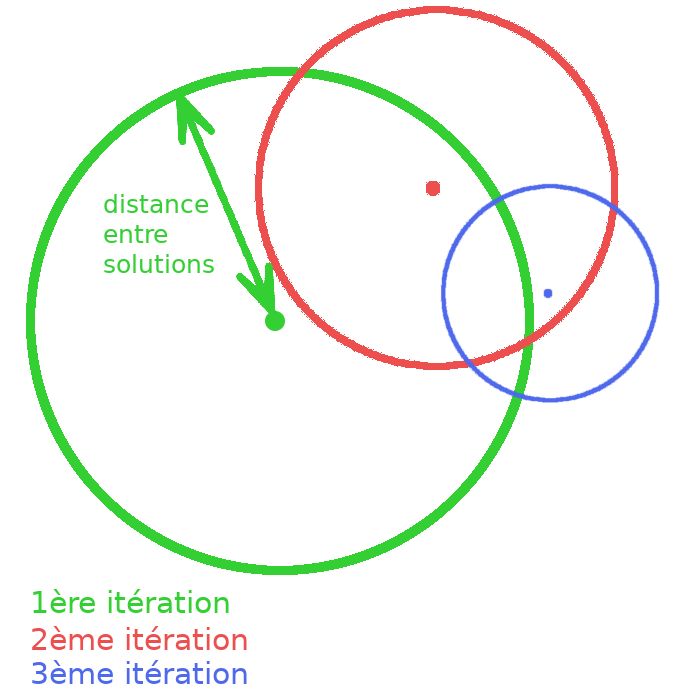
\includegraphics[scale=0.35]{images/imgs/regions.png}
		\caption{Illustration des régions de recherche des différentes itérations}
	\end{figure}
	\subsubsection{Nombre maximale d’itérations locale:}
	\paragraph{}
	Dans cette implémentation le nombre d’itération locale lui aussi varie en fonction de la distance. L’intuition était de choisir un nombre égale à la distance entre les solutions afin de mieux couvrir l’espace entre les elles tout en restant optimale par rapport au temps d’exécution. l’idée derrière c’est de donner la possibilité à la recherche locale d’arriver à toutes les solutions entre la solution sur laquelle on applique la recherche locale, et celle à partir de la quelle on a commencer l’itération de BSO.\\
	On peut illustrer un nombre d’itération locale égale à la distance comme suit:
	\begin{figure}[H]\label{localeSearch1}
		\centering
		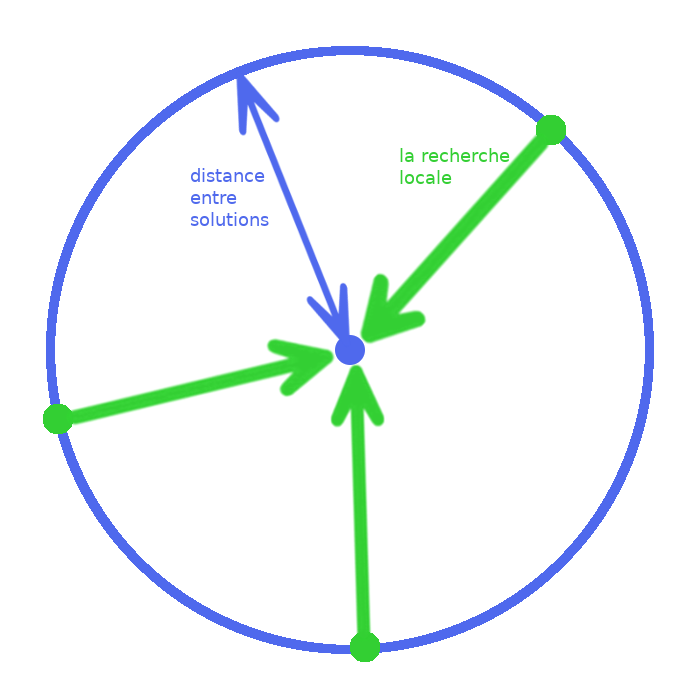
\includegraphics[scale=0.35]{images/imgs/localeSearch2.png}
		\caption{Illustration de BSO avec un nombre de recherche locale égale à la distance entre les solutions}
	\end{figure}
	Par contre dans le cas où le nombre d’itération locale est inférieur à la distance on ne pourra jamais arriver à la solution initiale puisque la recherche locale change un bit chaque itération, et pour arriver à la solution initiale on doit changer un nombre de bits égale à la distance entre les deux solutions. 
	\begin{figure}[H]\label{localeSearch2}
		\centering
		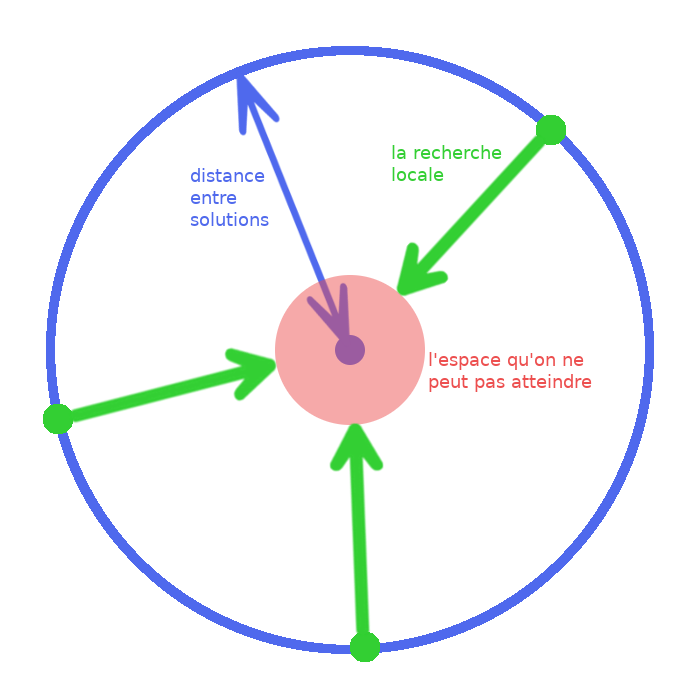
\includegraphics[scale=0.35]{images/imgs/localeSearch.png}
		\caption{Illustration de BSO avec un nombre de recherche locale inférieur à la distance entre les solutions}
	\end{figure}
	\paragraph{}
	Dans la suite de ce rapport nous allons comparer les deux implémentations entre elles expérimentalement ainsi qu’avec les solutions heuristique vu dans le premier chapitre. 
%%Amaze me here bro
